
\section{Time series model}
\label{sec:model:TSMS}

Following the traditional database models, a \acro{TSMS} model
consists of two components: a data model and a set of
operations. \emph{Measures} and \emph{time series} are the main
objects of our \acro{TSMS} model.
%
In this section, we describe and formalise the \acro{TSMS} model. 


\subsection{Data model}

Roughly speaking a \emph{time series} is a set of observations
collected at specific time instants. An observation may consist of a
single value or multiple values collected at the same time instant. We
refer a pair of time and observed values as a \emph{measure}. Then, a
time series is a correspondence between times and
values. Additionally, time series are also described as a set of
measures.

We name \emph{time domain} the set $\cal{T}$ of all the possible time
values. $\cal{T}$ can be either a finite or an infinite set and
usually it is a closed set. Although time is a complex issue
\cite{iep:time-supplement}, in this paper we will assume that
$\cal{T}$ is the set of affinely extended real numbers $\Rb = \R \cup
\{+\infty,-\infty\}$. This assumption avoids the complex details of
time modelling while being powerful enough for our purposes. Next, we
define the main time-related concepts using this naive approximation.

\begin{definition}[Time concepts]
  \label{def:model:temps}
  Let $\cal{T}=\Rb$ be the domain of time. We name an element
  $t\in\cal{T}$ as \emph{time instant}. Let $s,t\in\cal{T}$ be two
  time instants.  We define the \emph{duration of time} between $s$
  and $t$ as the value $d\in\cal{T}$ which measures the distance in
  time units between the two time instants, that is $d =|s-t|$.
\end{definition}

The \emph{value} is an attribute that indicates the magnitude of a
measure. The domain for the values can be of any data type. Valid
domains for values include integers, real numbers, strings, and richer
data structures such as arrays, lists, or even other time series. In
the sequel, the domain for values will be denoted by
$\cal{V}$. Without loss of generality, in this paper we will assume
that the domain of values is the set of projectively extended reals
$\Rp = \R \cup \{\infty\}$.

A measure represents an actual value measured at a particular time
instant. We define it below.

\begin{definition}[Measure]
  Let $v\in\cal{V}$ be a value and let $t\in\cal{T}$ be the time
  instant when the value was acquired. We define a \emph{measure} $m$
  as the tuple $m=(t,v)$. The domain of a measure $m$, written as
  $\dom m$, is the domain of its value.
\end{definition}

Let $m = (t,v)$ be a measure. In what follows, $V(m)$ denotes the
value $v$ and $T(m)$ denotes the time $t$.

Order between measures plays a significant role. Given two measures we
define two distinct \emph{order relations}.

\begin{definition}[Semitemporal order]\label{def:semitemporal_order}
  Let $m$ and $n$ be two measures. We name \emph{semitemporal order}
  the binary relation written $m\leq n$, defined as $m\leq n\iff
  (T(m)<T(n) \vee ( T(m)=T(n) \wedge V(m) = V(n) ))$.
\end{definition}

\begin{definition}[Temporal order]\label{def:temporal_order}
  Let $m$ and $n$ be two measures. We name \emph{temporal order} the
  binary relation written $m \leq^t n$ and defined as $m \leq^t n \iff
  T(m) \leq T(n)$.
\end{definition}

Note that the semitemporal order is a partial order and the temporal
order is a total order.


Intuitively speaking, a \emph{time series} is a ordered set of
measures of the same phenomena.  Sometimes they are also called
\emph{time sequences}~\cite{last:hetland}. We define it as follows.

\begin{definition}[Time series]
  \label{def:model:timeseries}
  Let $S = \{m_0,\ldots,m_k\}\subset\cal{T}\times\cal{V}$ be a finite
  set of measures of the same type. Then, $S$ is a \emph{time series}
  iff $\forall i,j: i,j\in[0,k] \wedge i\neq j: T(m_i)\neq T(m_j)$. We
  define the domain of a time series $S$ as the domain of its
  measures, denoted by $\dom S$.
\end{definition}

Observe that although measures in $S$ are expected to be of the same
phenomenon, from a formal standpoint we only require the domain of all
values to be the same.

A time series does not contain two measures at the same time. Therefore,
taking account of the temporal order, a time series is a totally
ordered set.

The \emph{cardinality} of a time series $S=\{m_0,\dots,m_k\}$, noted
as $|S|$, is the number of measures that it contains.  An \emph{empty
  time series} is noted as $\emptyset$. Needless to say,
$|\emptyset|=0$.

Although we defined values as scalars, it is easy to extend the
concept. Following~\cite{assfalg08:thesis}, a time series can record
more than one phenomenon if they share the same acquisition time
instants.  This kind of series is known as \emph{multivalued time
  series}. Let $S$ be a multivalued time series and let its domain be
$\dom S={\cal{V}}_1\times\cdots\times{\cal{V}}_n$. Then, we write its
measures as $m=(t,v_1,v_2,\ldots,v_n)$.

A time series is \emph{regular} when its measures are evenly spaced in
time, according to \cite{last:hetland}.  Let $S=\{m_0, m_1,\ldots,
m_{k-1},m_k\}$ be a time series, where
$T(m_0)<T(m_1)<\dots<T(m_{k-1})<T(m_k)$, and let $d\in\cal{T}$ be a
time duration. Then $S$ is \emph{regular} when $d=T(m_1)-T(m_0)=\dots
=T(m_k)-T(m_{k-1})$.

\subsection{Operations}
\label{sec:model:operations}

We can manipulate time series using the operations defined in this
section. Like the relational model operations, operations over time
series ignore the actual semantics of the data. In a real application,
it should be decided whether an operation is semantically coherent or
not and thus if it should be applied. For example, the addition of
values coming from two different phenomena could be semantically
wrong.

In this section, we formalise three groups of operations, one in each
of the subsections that follow. The set operations, that consider
times series as sets; the sequence operations, that consider time
series as sequences; and the temporal operations, that manipulate the
time series assuming they are representations of functions.


\subsubsection{Set operations}
\label{sec:set}

In what follows, we describe how to apply common set operators to time
series. We rely on how the relational model of \acro{DBMS} describes
operations based on set algebra~\cite{date:introduction}.

Consider a time series $S$. $S$ is a finite ordered set (by the
temporal order). Then, if $S$ nonempty, $S$ has a maximum and a
minimum.  The \emph{maximum} of $S$, denoted as $\max S$, is an
element of $S$ such that $\forall m \in S:\max S\geq^t m $. Because
$\max S$ is not defined when $S=\emptyset$, we are interested in the
concept of supremum.

Recall that the time domain is the set of affinely extended real
numbers $\Rb$. Then, for an empty subset $T=\emptyset$ of $\Rb$ we
know that its supremum is $\sup(T)=-\infty$
\cite{cantrell:extendedreal}.

Following the affinely extended reals, we apply the concept of
supremum to sets of measures, i.e., time series.

Assume that $m$ is an infinite measure.  To be consistent with the
affinely extended reals supremum, we consider $T(m)=-\infty$. $V(m)$
could be any arbitrary value. However, we choose an infinite value for
simplicity.
%
Then, we define an infinite measure $m$ as $m=(-\infty,\infty)$.

Henceforth, we say that the \emph{supremum} of a time series $S$,
noted as $\sup S$, is
\[
\sup S =\begin{cases}
  \max S              & \text{when $S$ nonempty}\\
  (-\infty,\infty)    & \text{otherwise}
\end{cases}
\]
Dually, we can define the \emph{minimum} of $S$, noted as $\min S$,
and the \emph{infimum} of $S$, noted as $\inf S$.

The \emph{membership} operation defines when a measure belongs to a
time series. We define two distinct membership operations which
consider the semitemporal order
(Definition~\ref{def:semitemporal_order}) and the temporal order
(Definition~\ref{def:temporal_order}). 
%
The two distinct membership definitions will induce two different ways
to consider time series and its operations.

Let $S$ be a time series and $m$ be a measure. We say that $m$ belongs
to $S$ (plain \emph{membership}), denoted as $m \in S$, when $\exists
x\in S: x=m$.  We also say that $m$ belongs temporally to $S$
(\emph{temporal membership}), denoted as $m \inst S$, when $\exists
x\in S : T(m)=T(x)$.

The two distinct membership criteria induce two meanings for
inclusion. Let $R$ and $S$ be two time series.  We say that $R$ is
\emph{included} in $S$, written $R\subseteq S$, when all the elements
of $R$ belong to $S$.  Analogously, we say that $R$ is \emph{included
  temporally} in $S$, noted $R\subseteqt S$, when all the elements of
$R$ belong temporally to $S$.

The \emph{union} of two sets is a set containing elements from both
sets. The traditional set union operations do not apply to time series
because the result time series may have repeated time values.  Thus,
we give a slightly modified concept for the union.

The union operation requires both time series to have the same domain,
as is also true with the union operation of relational
algebra~\cite{date:introduction}.

Let $R$ and $S$ be two time series and let $\dom R =\dom S$.  The
\emph{union} of $R$ and $S$, noted $R\cup S$, is a new time series $R
\cup S = \{m|m\in R\vee (m\in S\wedge m \notinst R)\}$.  The
\emph{temporal union} of $R$ and $S$, noted $R \cupt S$, is a time
series $R \cupt S = \{ m | (m \in R \wedge m \in S) \vee (m \in R
\wedge m \notinst S) \vee (m \in S \wedge m \notinst R) \}$.  It is
interesting to emphasise that the union is a non-commutative operation
while the temporal union is a commutative one.

\begin{figure}
  \centering
  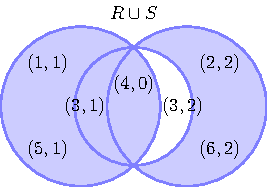
\includegraphics{fig_model_venn.pdf}
  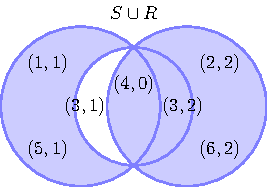
\includegraphics{fig_model_venn_reverse.pdf}
  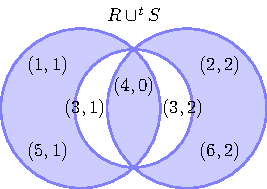
\includegraphics{fig_model_venn2.pdf}
  \caption{Venn diagrams for set and temporal set union operations of
    \acro{TSMS}}
  \label{fig:model:venn}
\end{figure}

\begin{example}\label{ex:model:s1s2}
  Let $R=\{(1,1), (3,1), (4,0), (5,1)\}$ and $S=\{(2,2), (3,2), (4,0),
  (6,2)\}$ be two time series. The union of $R$ and $S$ is $R\cup
  S=\{(1,1), (2,2), (3,1), (4,0), (5,1), (6,2)\}$. Because union is
  not symmetric, $S\cup R=\{(1,1), (2,2), \allowbreak(3,2), (4, 0),
  (5,1), (6,2)\}$. The temporal union results in $R\cupt S= S \cupt
  R=\{(1,1), (2,2), (4,0), (5,1), (6,2)\}$.
  %
  Figure~\ref{fig:model:venn} shows Venn diagrams for all three cases,
  where the coloured area depicts the result time series. In every
  diagram, the central intersection area contains measures that share
  both time and value attributes, as it is measure $(4,0)$. The left
  central area contains the measures in $R$ that only share the time
  attribute with a measure in $S$, as it is measure $(3,1)$. The right
  central area has a symmetrical meaning. The left and right outer
  areas are the remaining measures of $R$ and $S$ respectively.
\end{example}

Time series \emph{difference} can also be defined. Similar to the
union, the difference requires both time series to have the same
domain. Let $R$ and $S$ be two time series and let $\dom R = \dom
S$. The \emph{difference} between $R$ and $S$, written $R-S$, is a
time series $R-S=\{m|m\in R\wedge m\notin S\}$. The \emph{temporal
  difference} between $R$ and $S$, denoted $R-^t S$, is a time series
$R-^t S=\{m|m\in R\wedge m \notinst S\}$.

Based on union and difference we can define \emph{intersection} as
$R\cap S = R - (R - S)$ and \emph{symmetric difference} as $R \ominus
S = (R - S) \cup (S - R)$. We can also define the corresponding
temporal operations.

Relational \acro{DBMS} extend the set operators by some more, such as
selection, rename or join. This kind of operators also makes sense for
time series. To illustrate this possibility we define the join
operator.

Roughly speaking, the join of two time series is the combination of
measures sharing the same time attribute.  Let $R$ and $S$ be two time
series.  The \emph{join} of $R$ and $S$, denoted $R \join S$, is a
multivalued time series $R \join S = \{ (t,v_1,v_2) | (t,v_1) \in
R\wedge (t,v_2) \in S\}$. Note that $\dom(R\join S)=\dom R\times\dom
S$.  Noted that join requires both time series measures to share
exactly the same times. When time series diverge, the temporal
function operations explained later can be applied to adjust the time
instants to join requirements.

A \acro{DBMS} requires computational operators to enable calculations
between pieces of data. Relational \acro{DBMS} supply operators such
as extend, aggregate or summarise~\cite{date:introduction}. For time
series, we define the more general computational operators \emph{map}
and \emph{fold}.

The map operator transforms a time series $S$ into a new time series
$R$ by applying a function to every measure.  Let $S$ and $R$ be two
time series, let $\cal{V}=\dom S$ and $\cal{V'}=\dom R$, and let
$f:\cal{T}\times\cal{V}\rightarrow\cal{T}\times\cal{V'}$ be a function
over a measure returning a measure. The \emph{map} of $f$ over $S$ is
a new time series defined as $\map(S,f)=\{f(m)|m\in S\}$. Note that
$\dom(\map(S,f))=\cal{V'}$. 
In order to be as generic as possible, we do not impose any
restrictions on defining $f$. As a consequence, when $f$ operates with
time attributes the result of the map operation may be invalid as a
time series. However, when $f$ only operates with value attributes the
result is always valid. Therefore, the user must assure the proper
definition for $f$.



The fold operator recursively combines every measure of a time
series. Assuming that $\mathcal{P}(C)$ is the powerset of $C$, we
define fold as follows.
%
Let $S=\{m_0,\dots, m_k\}$ and $R$ be two time series, let
$\mathcal{V}=\dom S$, let $\mathcal{V'}=\dom R$ and let
%
$f:\mathcal{P}(\mathcal{T}\times\mathcal{V'}) \times
(\mathcal{T}\times\mathcal{V}) \rightarrow
\mathcal{P}(\mathcal{T}\times\mathcal{V'})$
%
be a function over a time series and a measure, which returns a time
series.
%
The \emph{fold} of $S$ by $f$ with initial value $R$ is a new time
series defined as $\fold(S,R,f) = f(\cdots(f(f(f(R,m_0),\allowbreak
m_1),\allowbreak m_2)\cdots),\allowbreak m_k)$.


The classical aggregation operator combines the data of a time series
into a single value.  It is worth noting that it is a special case of
fold.

Let $S=\{m_0,\dots,m_k\}$ be a time series, let $\mathcal{V}=\dom S$,
let $m$ be a measure with $\dom m=\mathcal{V}$, and let
$f:(\mathcal{T}\times\mathcal{V})\times(\mathcal{T}\times\mathcal{V})\rightarrow
\mathcal{T}\times\mathcal{V}$ be a function over two measures
returning a measure. The \emph{aggregate} of $S$ by $f$ with initial
value $m$ is a new time series defined as $\agg(S,m,f) =
f(\cdots(f(f(f(m,m_0),\allowbreak m_1),\allowbreak
m_2)\cdots),\allowbreak m_k)$.


\begin{example}
\label{ex:computational-operators}
Let $S=\{(1,1),(2,3),(4,1)\}$ be a time series.  Map operator allows
computing a new time series whose values result from time attribute
plus a duration of time.  We define the map function
$f(t,v)=(t,t+5)$. Then $\map(S,f)=\{(6,1),(7,3),(9,1)\}$. As we will
use it later, we name this operation \emph{translation} of a time
series.

The fold operator allows, for instance, to select the measures having
its value equal to one.  We define the fold function $f(R,m)=R\cup R'$
where $R'=\{m\}$ if $V(m)=1$ or $R'=\emptyset$ otherwise. Let $m$ be
any measure, note that $f(\emptyset,m)= R'$. Then
$\fold(S,\emptyset,f)=\{(1,1),(4,1)\}$.

The aggregate operator allows, for example, to compute the measure
that results from the sum of all the values.  To illustrate it, we
define the aggregate function $f(m,n)=(0,V(m)+V(n))$. Now,
$\agg(S,(0,0),f) = (0,5)$, where $5$ is the sum of all the values of
$S$. Note that time is meaningless in this computation.
\end{example}

%%%%%%% BINARY COMPUTATIONAL OPERATORS

Finally, we describe how using the operators defined before, we can
implement \emph{binary computational} operators between two time
series. This implementation illustrates the power of the operators
defined so far.

The strategy requires first to join the two time series and then apply
the computational operations. Let $S$ and $R$ be two time series and
$\odot$ be a binary operator on the value domain. We can extend the
operator $\odot$ to the time series as $S\odot R=\map(S\join R, f)$
being $f$ the function $f(t,v,w)=(t,v\odot w)$. The extended operator
allows to extend real binary operations such as sum, $R+S$, to time
series.

\begin{example}
  \label{ex:model:sum}
  Let $R=\{(1,2), (2,2), (4,0)\}$ and $S=\{(1,1), (2,2), (4,1)\}$ be
  two time series.  The sum of $R$ and $S$ is defined as
  $R+S=\map(S\join R, f)$ being $f$ the function $f(t,v,w)=(t,v+ w)$.
  Then the sum results $R+S= \{(1,3), (2,4), (4,1)\}$.
\end{example}

As binary computational operators depend on join operator, it must be
recalled that join requires both time series measures to share exactly
the same times. As aforementioned, when time series diverge, the
temporal function operations explained later can be applied to adjust
the time instants to join requirements.



\subsubsection{Sequence operations}
\label{sec:sequence}

Sequence operations manipulate time series considering measures as
being totally ordered by time.  We define three basic operations:
\emph{slice}, \emph{successor} and \emph{concatenation}.

The classical interval concept can be applied to the time domain. In this
context, given two time instants $s$ and $t$, we use the notation
$[s:t]$, $(s:t)$, $[s:t)$ and $(s:t]$ respectively for the closed
interval, open interval, right open and left open interval.
%
Following~\cite{last:hetland}, to slice a time series $S$ means to
extract a new time series $R\subseteq S$ constrained to a given time
interval. We denote this operation as the original time series followed
by the interval. Therefore, $S[s:t]=\{m|m\in S \wedge
T(m)\in[s:t]\}$. We can use other intervals to slice a time series in
the same fashion. For instance, $S(s:t]=\{m|m\in S \wedge
T(m)\in(s:t]\}$.

The ordinary time order allows to define the concepts of successor and
predecessor for the measures of a time series.
%
Let $S=\{m_0,\ldots,m_k\}$ be a time series and $m$ be an arbitrary
measure.
%
We say that $m_i=\nex_S(m)$ is the measure \emph{next} to $m$ in $S$
if and only if $m_i=\inf(S(T(m):+\infty])$.
%
We also say that $m_i=\prev_S(m)$ is the measure \emph{previous} to
$m$ in $S$ if and only if $m_i=\sup(S[-\infty:T(m)))$.
%
Infinite measures are obtained when next and previous are applied to
supremum and infimum measures respectively: $\nex_S(\sup
S)=(+\infty,\infty)$ and $\prev_S(\inf S)=(-\infty,\infty)$.

To concatenate two time series means to compute a new time series with
the measures of the first time series followed in time order by the
measures of the second one. 
%
The concatenation requires both time series to share the same domain.
Let $R$ and $S$ be two time series and let $\dom R=\dom S$. The
\emph{concatenation} of $R$ and $S$, denoted as $R||S$, is a time
series that contains all the measures of $R$ together with those of
$S$ that do not intersect with the time interval of $R$. That is,
$R||S= R\cup (S - S[T(\inf R):T(\sup R)])$.



\subsubsection{Temporal function operations}
\label{sec:model:tfunc}

We can think a time series as a discrete representation of an original
temporal function. In this section, we devise some operations that
manage time series according to this point of view.

Let $S$ be a time series. A \emph{temporal representation function} is
a function $S$ defined as $S:\Rb\rightarrow\cal{V}$
%%%%%%%%%%%%%%%%%%%%%%%%%%%%%%%%%%%%%%%%%%%%%%%%%%%%%%%%%%%%%%%%%%%%%%%
%%%%%%%%%%%%%% REPASSAR ALEIXXXX IMPORTANT!!!!!
such that for every measure $m\in S$, $V(m)=S(T(m))$.
%%%%%%%%%%%%%%%%%%%%%%%%%%%%%%%%%%%%%%%%%%%%%%%%%%%%%%%%%%%%%%%%%%%%%%%
In some sense, we can think of $S(t)$ as the original temporal
function from which $S$ was obtained.

The graph of a function allows to obtain and interpret the continuous
nature of a time series. When we can plot the domain of time and value
attributes, then the graph is equivalent to a graphical
representation.
%
Let $S$ be a time series and let $\cal{T}$ be the time domain. The
\emph{graph} of the time series $S$ is a set of ordered pairs $\graph
S =\{(t,S(t))|t\in \cal{T}\}$ where $S(t)$ is a temporal
representation function for the time series.

There is not an unique way to obtain $S(t)$ for a given time series
$S$. Because of this, in temporal representation functions we will
introduce a superscript that shows the name $r$ of the representation
method used. Then, $S(t)^r$ means the representation function of $S$
using method $r$. Below, we exemplify the representation functions
using two different methods based on impulse and constant piecewise
functions.

\begin{definition}[Dirac representation] 
  Dirac delta (\dd) is a method of representation based on the Dirac
  delta function. Let $S$ be a time series. We define $S(t)^\dd$ as
  the following \dd{} representation function:
  \[
  S(t)^\dd
  =  \begin{cases}
          V(m) & \text{if } \exists m\in S:t=T(m) \\
          0    & \text{otherwise}
  \end{cases}
  \]
\end{definition}

\begin{definition}[Zohe representation]
  Zero-order hold everted (\zohe{}) is a method of representation
  based on the \emph{zero-order hold} signal reconstruction method. It
  is a piecewise constant function built from left-continuous step
  functions.  Let $S$ be a time series. We define $S(t)^\zohe$ as the
  following representation function:
  \[
  S(t)^\zohe 
  = \begin{cases}
    V(m) & \text{if } \exists m\in S: t\in \big(T(\prev_S(m)):T(m)\big]\\
    0    & \text{if } t > T(\max(S)) 
  \end{cases}
  \]
\end{definition}

We use the concept of representation to formalise some set and
sequence operators as temporal operators.

We define a temporal interval operation to introduce this concept.
Let $S$ be a time series, let $[s:t]$ be an interval of two time
instants and let $r$ be a representation method. The \emph{temporal
  interval}, denoted as $S[s:t]^r$, returns a new time series with
measures in the interval temporal range. That is, $S[s:t]^r = S(u)^r$
for all $u \in [s:t]$. This is a general definition difficult to
implement, so for every representation a particular temporal interval
must be interpreted:

\begin{itemize}
\item Let $S(t)^\dd$ be the \dd{} representation for $S$. The
  \emph{\dd{} temporal interval} is $S[s:t]^\dd = S[s:t]
  \cup \{m\} \cup \{n\}$ where $m=(s,0)$ and $n=(t,0)$.

\item Let $S(t)^\zohe{}$ be the \zohe{} representation for $S$. The
  \emph{\zohe{} temporal interval} is $S[s:t]^\zohe{} = S(s:t]
  \cup \{m\}$ where $m=(t,v)$ and $v= V(\inf( S[t:+\infty] ))$.
\end{itemize}

From temporal interval, we can define other operators such as temporal
selection, temporal concatenation, or temporal join. As an example, we
give the definition of the temporal selection and the temporal join
operations.

The temporal selection over a time series allows to change the
resolution in the context of a representation function.  Let $S$ be a
time series, let $T=\{t_0,t_1,\dotsc,t_k\}$ be a set of time instants,
and let $r$ be a representation method. The \emph{temporal selection},
denoted as $S[T]^r$, is a time series of measures in $T$ and times
computed in coherence with the representation method $r$. That is,
$S[T]^r = S[t_0:t_0]^r \cup S[t_1:t_1]^r \cup \dotsb \cup
S[t_k:t_k]^r$. If $t$ is a time instant, note that the temporal
selection depends on the temporal interval operation $S[t:t]^r$, which
is equivalent to the notion of temporal representation function over a
single time instant. That is, $S[t:t]^r = \{ (t, S(t)^r) \}$.

The temporal selection operation also allows to regularise an
irregular time series. Let $S$ be a time series, let $d,e\in\cal{T}$
be the desired regularity parameters, and let $k\in\N$ be a limit for
the scope of the range.  A regularised $S$ can be obtained with
$S[T]^r$ where $T = \{e+nd | n\in\N \wedge n\leq k \}$ is a set of
evenly spaced time instants.


Another use case for the temporal selection is for joining two time
series that do not share the same times. Let $R$ and $S$ be two time
series that do not share times, i.e. their time sets are dissimilar
$\{t | (t,v) \in R\} \neq \{t | (t,v) \in S\}$. Then, we can not apply
the previously defined $R \join S$.  However, we can define a more
elaborated join based on the temporal selection, which we name
\emph{temporal join}.  Let $r$ be a representation method and let
$T=\{t | (t,v) \in R\} \cup \{t | (t,v) \in S\}$ be the union of both
time sets.  The \emph{temporal join}, denoted as $R \join^r S$,
returns a new time series $R \join^r S = R[T]^r \join S[T]^r$.

Using temporal join, we can also solve binary computational operation
for time series that have dissimilar time sets. Next, we redo
Example~\ref{ex:model:sum} to extend sum binary computational
operation with temporal join.

\begin{example}
  \label{ex:m:sumtemporal}
  Let $R=\{(1,2), (2,2), (4,0)\}$ and $S=\{(1,1), (3,2), (4,1)\}$ be
  two time series and let $r=\zohe{}$ be a representation method.  
  The sum of $R$ and $S$ is defined as $R+S=\map(S\join^r R, f)$ being
  $f$ the function $f(t,v,w)=(t,v+ w)$.

  The union of both time sets is $T=\{1,2,3,4\}$. The corresponding
  temporal selection over both time series is $R[T]^r=\{
  (1,2),\allowbreak (2,2), (3,0),\allowbreak (4,0)\}$ and
  $S[T]^r=\{(1,1),\allowbreak (2,2),\allowbreak (3,2), (4,1)\}$.  The
  temporal join of both is $R \join^r S=\{ (1,2,1),\allowbreak (2,2,2), (3,0,2),
  (4,0,1)\}$.  Then the sum results $R+S= \{(1,3),\allowbreak (2,4), (3,2),
  (4,1)\}$.
\end{example}




\section{Multiresolution model}
\label{sec:MTSMS}

In Section~\ref{sec:features} we intuitively introduced the concept of
multiresolution through an example. In this section, we formalise a
model for \acro{MTSMS}. At the end of the section, we will offer some
illustrative examples of the previous formalisation.

A \acro{MTSMS} is a \acro{TSMS} that stores time series using a lossy
compression approach. The \acro{MTSMS} model is based on the concepts
of \emph{measures} and \emph{time series} as defined in
Section~\ref{sec:model:TSMS}.  A \acro{MTSMS} stores a time series as
a structure that we call \emph{multiresolution time series}. A
multiresolution time series is a collection of \emph{resolution
  subseries} that store a view of the original time series in a given
resolution. The operator that adds data to a resolution subseries
requires accumulating transient measures in a \emph{buffer}. This
procedure allows to aggregate original data to obtain the expected
resolution and finally store them in a \emph{disc}.


\begin{figure}
  \centering
  %\begin{tikzpicture}
 \tikzset{
        myarrow/.style={->, >=latex',  thick},
      }
      

  \node[rectangle,draw,minimum height=6cm,minimum width=9cm] (m) {};
  \draw[shift=( m.south west)]   
  node[above right] {base de dades multiresolució};


  %discmig
  \node (m.center) (discr1) {...};

  %discr
  
  \node[ellipse,draw,minimum height=3.5cm,minimum width=2.5cm,alias=discr0] [left=of discr1] {};
  \node[above=0cm of discr0.north] {R0};
  \node[below=0cm of discr0] {disc resolució};

  \node[cylinder, draw, shape border rotate=90, aspect=0.25,alias=buffer0] [below=3mm of discr0.north] {buffer};
  \node[circle, draw,alias=disc0]  [above=3mm of discr0.south] {disc} ;
  \draw [->] (disc0.center)++(.4:.4cm) arc(0:180:.4cm);
  \draw[myarrow] (buffer0.bottom) -- (disc0.north);


  %discrd

  \node[ellipse,draw,minimum height=3.5cm,minimum width=2.5cm,alias=discrd] [right=of discr1] {};
  \node[above=0cm of discrd] {Rd};
  \node[below=0cm of discrd] {disc resolució};

  \node[cylinder, draw, shape border rotate=90, aspect=0.25,alias=bufferd] [below=3mm of discrd.north] {buffer};
  \node[circle, draw,alias=discd]  [above=3mm of discrd.south] {disc} ;
  \draw [->] (discd.center)++(.4:.4cm) arc(0:180:.4cm);
  \draw[myarrow] (bufferd.bottom) -- (discd.north);



  %mesura 
  \node[above=1cm of m.north] (m0) {};

  \draw[myarrow] (m0) -- (m.north) 
  node[right,midway] {mesura};

  \draw[myarrow] (m.north) -- (buffer0);
  \draw[myarrow] (m.north) -- (bufferd);
  \draw[myarrow] (m.north) -- (discr1);

\end{tikzpicture}
  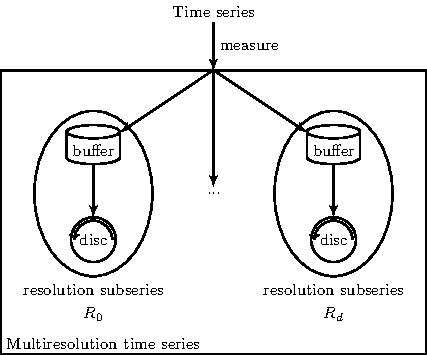
\includegraphics{fig_model_mtsdb.pdf}
  \caption{Architecture of \acro{MTSMS} model}
  \label{fig:model:mtsdb}
\end{figure}

Figure~\ref{fig:model:mtsdb} shows the architecture of a \acro{MTSMS}
for a single multiresolution time series. The original time series
gets stored in multiple resolution subseries. Each resolution
subseries has a particular time resolution and attribute aggregation
policy. Discs are size bounded so they only contain a fixed amount
of measures. When a disc becomes full, it discards a measure. Thus, a
multiresolution database is bounded in size and the time series gets
stored in several storage bounded time subseries.

Regarding operations, the \acro{MTSMS} model requires two kinds of
operators. Some operators should be devoted to set up the time
intervals between measures and to aggregate the attributes. Some other
operators should be dedicated to query the multiresolution schema and
to extract the time series data.

Following, we define the \acro{MTSMS} model structure, its structural
operators, the operations to query a multiresolution time series, and
the \emph{attribute aggregate functions}.  Although schema
manipulation operations could be defined, in this paper we exclusively
focus on structure and data query operators.


\subsection{Structure}

A \emph{buffer} is a container for a time series. The aim of a buffer
is to regularise the time series using a constant \emph{resolution
  step} and an \emph{attribute aggregate function}.  We name the
regularisation action as \emph{consolidation}. We defined the
attribute aggregate functions in Section~\ref{sec:model:interpolador}.

\begin{definition}[Buffer]
  Let $S$ be a time series, let $\tau\in\cal{T}$ be the last
  consolidation time, let $\delta\in\cal{T}$ be the resolution step
  and let $f$ be an attribute aggregate function. We define a
  \emph{buffer} $B$ as the tuple $B=(S,\tau,\delta,f)$.
\end{definition}

An empty buffer $B$ is defined as $B=(\emptyset, t_0, \delta, f)$,
i.e., an empty time series, an initial consolidation time
$t_0\in\cal{T}$, a resolution step $\delta$, and a function $f$.
Given a buffer, all the consolidation time instants can be determined
as $\tau_n=t_0+n\delta$ for all $n\in\N$.

Let $B=(S, \tau, \delta, f)$ be a buffer. The \emph{consolidation} of
$B$ is an operation that computes a new measure $m=f(S, \tau, \delta)$
summarising the data of $S$ comprised in the given interval.

A buffer has two main structural operations. The first one adds a
measure to the buffer, and the second one consolidates the buffer.

Let $B=(S,\tau,\delta,f)$ be a buffer and let $m$ be a measure.  The
addition of $m$ to $B$, noted as $\addB(B,m)$, returns a new buffer
$\addB(B,m)=(S',\tau,\delta,f)$ where $S' = S \cup \{m\}$.

Let $B=(S,\tau,\delta,f)$ be a buffer. The consolidation of $B$, noted
as $\consB(B)$, returns a new buffer and a new measure $\consB(B)=
(B',m')$ where $B'= (S[\tau+\delta:+\infty], \tau+\delta,\delta,f)$
and $m' = f(S,\tau,\delta)$. After the consolidation, we can remove
from the buffer the consolidated part of the time series. Therefore,
we discard historical data.

We apply the consolidation of a buffer to the first non-consolidated
time instant. We obtain the total consolidation by successive
applications of the operator. Consolidation requires the measures to
be added by time order and to consolidate the buffer when the time of
some measure is bigger than the buffer's next consolidation time.  Let
$B=(S,\tau,\delta,f)$ be a buffer, and let $m=\sup S$ be the maximum
measure of $B$. We say that $B$ is consolidable if and only if $T(m)
\geq \tau+\delta$.

A \emph{disc} is a finite capacity container of measures. A time
series stored in a disc has its cardinal bounded. When the cardinal of
the time series is to overcome the limit, some measures need to be
discarded.

\begin{definition}[Disc]
  Let $k\in\N$ and $S$, $|S|\leq k$, be a time series. We define a
  \emph{disc} $D$ as the tuple $D=(S,k)$.
\end{definition}

An empty disc is noted as $(\emptyset,k)$. It is the tuple of an empty
time series and a bound $k$.

The main operation on a disc is to add a measure while keeping under
control the cardinal of the times series. Let $D=(S,k)$ be a disc and
let $m$ be a measure.  The addition of $m$ to $D$, written as
$\addD(D,m)$, is a new disc $\addD(D,m)=(S',k)$ where
\[
S' = \begin{cases}
  S\cup\{m\}                 & \text{if } |S|<k  \\
  (S-\{\min S\}) \cup \{m\} & \text{otherwise}
\end{cases}  
\]

A \emph{resolution subseries} is a structure that regularises and
aggregates a time series. This structure is composed of a buffer,
which contains the time series to be regularised, and a disc, which
contains the regularised time series.

\begin{definition}[Resolution subseries]
  Let $B$ be a buffer and let $D$ be a disc.  We define a
  \emph{resolution subseries} $R$ as the tuple $R=(B,D)$.
\end{definition}
 
The operators of a resolution subseries extend the buffer and disc
ones. Let $R=(B,D)$ be a resolution subseries, and let $m$ be new a
measure.  The addition of $m$ to $R$, noted as $\addR(R,m)$, is a new
resolution subseries $\addR(R,m)=(B',D)$ where $B'= \addB(B,m)$ is the
addition of the measure to the buffer.  The consolidation of $R$,
noted as $\consR(R)$, is a new resolution subseries
$\consR(R)=(B',D')$, where $(B',m') = \consB(B)$ is the consolidation
of the buffer, and $D'= \addD(D,m')$ is the addition of the
consolidated measure to the disc. A resolution subseries is
consolidable only when its buffer is consolidable.

A \emph{multiresolution time series} is a set of resolution subseries
referred to the same time series. We store a time series regularised
with distinct resolutions across the resolution subseries, as
previously shown in Figure~\ref{fig:model:mtsdb}.

\begin{definition}[Multiresolution time series]
  Let $M=\{R_0, \dots, R_k\}$ be a finite set of resolution
  subseries. Then $M$ is a \emph{multiresolution time series}.
\end{definition}

Therefore, to define a multiresolution time series we must define the
number of resolution subseries and its corresponding parameters
$(\delta,\tau,f,k)$.  Usually, there are no repeated pairs of
$(\delta,f)$ parameters among a multiresolution series, so they act as
key attributes.

The operators of a multiresolution time series apply to every
resolution subseries contained. Let
$M=\{R_0,\allowbreak\dots,\allowbreak R_k\}$ be a multiresolution time
series and let $m$ be a measure. The addition of a measure to every
resolution subseries, noted as $\addM(M,m)$, is a new multiresolution
time series $\addM(M,m)=\{R'_0, \dots,\allowbreak R'_k\}$ where
$R'_i=\addR(R_i,m)$. The consolidation of all resolution subseries,
noted as $\consM(M)$ is a new multiresolution time series
$\consM(M)=\{R'_0,\allowbreak\dots,\allowbreak R'_k\}$ where
\[R'_i=
\begin{cases}
\consR(R_i) & \text{if } R_i \text{ consolidable}\\
 R_i & \text{otherwise}
\end{cases}
\]


\subsection{Queries}

There are two basic time series queries for a \acro{MTSMS}: a query to
extract a time subseries from a resolution subseries, and a query to
obtain a total time series from all consolidated data.

Let $M$ be a multiresolution time series and let $(\delta,f)$ be a
pair of key attributes.  The query operator denoted as
$\seriedisc(M,\delta,f)$ computes a time series such that $\exists
(B,D) \in M: B=(S,\tau,\delta,f) \wedge D=(\seriedisc(M,\delta,f), k)
$ where $S,\tau,k$ are bound variables.  We assume that there are no
repeated $(\delta,f)$ pairs in $M$.

Recall that $R||S$ is the concatenation of two time series
$R$ and $S$, which we defined in Section~\ref{sec:sequence}.

Let $M=\{R_0,\dots,R_k\}$ be a multiresolution time series and let
$S_0, \dots, S_k$ be the time series corresponding to the resolution
subseries $R_0,\dots,R_k$. Assume that the attribute aggregation
functions of all $R_i$ are the same and the resolution steps of all
$R_i$ are distinct. 
%
We define the query operator $\totalseries(M)$, the time ordered
concatenation of all time subseries, as follows.
%
$\totalseries(M) = S_{i_0} || S_{i_1} || \cdots || S_{i_k}$
%
where $i_0,\dots,i_k$ is a permutation of $[0,k]$ such that
$\delta_{i_0} < \delta_{i_1} < \cdots < \delta_{i_k}$, being $\delta_i$
the resolution step of the resolution subseries $R_i$.

The operator $\totalseries$ obtains the better possible resolution.

Using these basic time series queries, we can define more elaborated
queries for an \acro{MTSMS} by using \acro{TSMS} operations. For
example, let $L$ and $M$ be two multiresolution time series with the
same multiresolution parameters. We can compute the sum of both as
$\totalseries(L) + \totalseries(M)$. Recall that $R+S$ is the sum of
the values of two time series $R$ and $S$ that we defined in
example~\ref{ex:model:sum} as a binary computational operator.


When two multiresolution time series do not have the same
multiresolution parameters, then $\totalseries(L) + \totalseries(M)$
must be solved using temporal join, as we showed in
Example~\ref{ex:m:sumtemporal}. Nevertheless, dealing with
temporal join operations can be cumbersome as they depend on a
representation method parameter. In this regard, we can consider some
multiresolution enhancements:

\begin{itemize}

\item If $L$ and $M$ share a resolution subseries with the same
  $\tau$ and $\delta$ parameters, then it is possible to compute
  $\seriedisc(L,\delta,f_1) + \seriedisc(M,\delta,f_2)$ with the basic
  join. The uninstantiated variables $f_1$ and $f_2$ are any attribute
  aggregate functions, although usually it makes more sense to be the
  same $f_1=f_2$.

\item If $L$ and $M$ share a resolution subseries with only the same
  $\delta$, then the previous point can be applied if one time
  subseries is be translated. Let $R=\seriedisc(L,\delta,f_1)$ and
  $S=\seriedisc(M,\delta,f_2)$ be the time subseries desired and let
  $\tau_R$ and $\tau_S$ be the corresponding last consolidation time
  for each $\delta$. Let $f(t,v)=(t,t+\tau_R-\tau_S)$ be a map
  function and let $S'=\map(S,f)$ be the result of the translation
  operation, as we showed in Example~\ref{ex:computational-operators}.
  Then, we can apply $R+S'$ with the basic join.
  
\item Otherwise, when $L$ and $M$ do not share any resolution
  subseries with the same $\delta$, the temporal join must be used in
  the sum $\totalseries(L) + \totalseries(M)$.  However, as $L$ and
  $M$ are lossy storage solutions for the original time series they
  represent, $\totalseries(L) + \totalseries(M)$ computes less data
  than applying the sum directly to the original time series.

\end{itemize}




\subsection{Attribute aggregate function}
\label{sec:model:interpolador}

Attribute aggregate functions are a particular case of \acro{TSMS}
aggregate operations used to summarise time series data while
consolidating a buffer.

Let $S$ be a time series, let $\delta$ be a resolution step and let
$\tau$ be a consolidation time.  An \emph{attribute aggregate
  function} $f$ calculates a new measure $m=f(S,\tau,\delta)$. From
$\tau$ and $\delta$, we obtain the time interval $[\tau:\tau+\delta]$.
Then, the resulting measure $m$ is interpreted to summarise the
measures of $S$ for the time interval $[\tau:\tau+\delta]$.

An attribute aggregation function follows this general scheme. First,
it obtains a time subseries $S'$ according to the consolidating
interval using a slice operator. For example, $S' =
S[\tau:\tau+\delta]$. Second, it applies a \acro{TSMS} aggregation
function on this time subseries to obtain $m$. For instance, $m =
\agg(S',n, f)$, being $f$ an aggregation function and $n$ an initial
measure, as defined in Section~\ref{sec:set}.

We can use many different attribute aggregate functions to summarise a
time series. For instance, it is possible to calculate a statistical
indicator of the time series such as the average or a more complex
digital signal processing operation as proposed
in~\cite{zhang11}. Furthermore, during the aggregation process we can
consider the representation of a time series and some of its
pathologies.

Given the diversity of attribute aggregate functions, no global
assumptions can be made about them. Each user should decide which
combination of aggregation and representation fits better to the
measured phenomenon.  Therefore, the \acro{MTSMS} model must have a
generic design that allows the users to define their aggregate
functions.

In what follows we will give some examples of usual attribute
aggregation functions. These functions compute a new measure given a
set of known measures. Then, an attribute aggregation function should
compute a new \emph{time} and a new \emph{value} from the set of known
measures.

Usually, an attribute aggregation function returns measures that match
the buffer consolidating times. Assume, for instance, that $f$ is an
attribute aggregation function and let $m=f(S,\tau,\delta)$.  Then,
the time of $m$ is usually computed as $T(m)=\tau+\delta$.  However,
in some cases it is preferable for $T(m)$ not to match the buffer
consolidating times. For instance, the resulting measure can be
aggregated from a time subseries $S'$ using an open interval
$S'=S(\tau:\tau+\delta)$, a closed interval $S'=S[\tau:\tau+\delta]$,
or other combinations as it is $S'=S(\tau-d:\tau+\delta-d]$, where $d$
is a time duration that delays the consolidation to
$T(m)=\tau+\delta-d$.  This time offset can also be variable. For
example, consider an aggregate function that returns the first measure
of the interval $m=\min(S[\tau:\tau+\delta))$, then the resulting time
fulfils that $\tau\leq T(m) < \tau+\delta$.

Assume that $f$ is an attribute aggregation function and let
$m=f(S,\tau,\delta)$.  An attribute aggregation function $f$ should
compute the value of $m$. Next, there are some examples that illustrate
how to compute $V(m)$ based on the temporal function time series
operators.  That is, the time series aggregated is interpreted by the
temporal representation function $S(t)^r$ as has been described in
Section~\ref{sec:model:tfunc}. In these example functions, we leave
the time series representation $r$ uninstantiated.

\begin{itemize}

\item The \emph{maximum} computes $V(m)$ as $V(m) =
  \max\limits_{\forall t \in [\tau:\tau+\delta]} S(t)^r$. It
  summarises $S$ with the maximum of the measure values in the
  interval $[\tau:\tau+\delta]$.

\item The \emph{last} computes $V(m)$ as $V(m) = S(\tau+\delta)^r$. It
  summarises $S$ with the value at $\tau+\delta$ time instant.

\item The \emph{mean} computes $V(m)$ as $V(m) = \frac{1}{\delta}
  \int\limits_{\tau}^{\tau+\delta} S(t)^r dt$. It summarises $S$ with
  the mean of the function in the interval $[\tau:\tau+\delta]$.

\end{itemize}

We can instantiate the time series representation in the previous
examples in several ways. In what follows, we exemplify this by
instantiating $r$ as \dd{} and \zohe{}.

Dirac delta attribute aggregation functions interpret the resulting
time as centered on the interval $T(m)=\frac{2\tau+\delta}{2}$. The
resulting value $V(m)$ depends on the attribute. Let
$S'=S[\tau:\tau+\delta]^\dd$ be the selection of measures by Dirac
delta temporal interval. Then,
\begin{itemize}
\item The $maximum^\dd$ is such that $V(m) =
  \max\big(0,\max\limits_{\forall n \in S'} V(n)\big)$.
\item The $last^\dd$ is such that $V(m) = V(\max S')$.
\item The $mean^\dd$ is such that $V(m) = \frac{1}{\delta}
  \sum\limits_{\forall n \in S'} V(n)$. Note that for the Dirac
  delta function $\int\dd(t)dt=1$.
\end{itemize}

Note that $\sum\limits_{\forall n \in S'} V(n)$ is a sum of values
that could be implemented as $\agg(S',(0,0),f)$ where
$f(m,n)=(0,V(m)+V(n))$, as shown in
Example~\ref{ex:computational-operators}.

\zohe{} attribute aggregation functions interpret the resulting time
as the right limit of the interval $T(m)=\tau+\delta$. The resulting
value $V(m)$ depends on the attribute, let
$S'=S[\tau:\tau+\delta]^\zohe{}$ be the selection of measures by
\zohe{} temporal interval. Then,

\begin{itemize}

\item The $\maxz$ is such that $V(m) = \max\limits_{\forall n \in S'}
  V(n)$.

\item The $last^\zohe{}$ is such that $V(m) = V(\max S')$.

\item The $\meanz$ is such that $V(m) = \frac{1}{\delta}
  \big[(T(o)-\tau)V(o) + \sum\limits_{\forall n\in R}( T(n)-
  T(\prev_S n) )V(n)\big]$ where $o=\min S'$ and $R= S' - \{o\}$.

\end{itemize}

Note that $\meanz$ is a sum of values that could be implemented as
$\meanz = \frac{1}{\delta}\agg(S',(0,0),f)$ where $f(m,n)=(0,V(m)+v)$
and
\[
 v=
 \begin{cases}
   (T(n)-\tau)V(n) & \text{if } n=\min S'\\
   (T(n)-T(\prev_{S'} n))V(n) & \text{else }
 \end{cases}
\]

\emph{RRDtool}, \cite{rrdtool}, uses an aggregation function similar
to $\meanz$ to summarise velocity counter data by keeping the area
below the original signal.

It is interesting to note that some attribute aggregation patterns are
very similar. For instance, the maximum and last attribute aggregation
schemes differ basically in the interval selection operation. However,
other patterns have a more elaborated interpretation depending on the
actual representation used, as it is the case of $\meanz$ and
$mean^\dd$.


To summarise the model we have formalised in this section, we show a
basic multiresolution example.
\begin{example}\label{ex:model:smultiresolution}
  We define a multiresolution schema for a time series, we consolidate
  the database and we query its data.  Let $S =
  \{(1,6),(5,2),\allowbreak (8,5),\allowbreak (10,0),\allowbreak
  (14,1),\allowbreak (19,6),\allowbreak (22,11),\allowbreak
  (26,6),(29,0) \}$ be a time series and let $M=\{R_0,R_1\}$ be a
  multiresolution time series where each resolution parameters are
  $\tau_0=0$ , $\delta_0=5$, $f_0 =\meanz$, $k_0=4$ and $\tau_1=0$,
  $\delta_1=10$, $f_1 =\maxz$, $k_1=2$. Therefore $R_0$ will be
  consolidated at time instants 5, 10, 15, 20, 25, 30\dots and $R_1$
  at 10, 20, 30\dots

  We add all measures of $S$ to $M$, and then we consolidate it until
  it is no more consolidable. As $T(\max S)=29$, the last
  consolidation times are $\tau_0=25$ and $\tau_1=20$, so let $M_{29}$
  be the multiresolution time series at this state.

  Then, the two time subseries consolidated are obtained by querying
  $\seriedisc(M_{29},5,\meanz) = \{(10,3), (15,2), (20,7), (25,8)\}$
  and $\seriedisc(M_{29}, 10,\allowbreak \maxz) = \{(10,6),
  (20,11)\}$. Regarding buffers, let $S_0$ and $S_1$ be the $M_{29}$
  buffer's time series, note that $S_0= \{(26,6), (29,0)\}$ and
  $S_1=\{(22,11), (26,6), (29,0)\}$.

  In this particular example, $ \totalseries(M_{29}) =
  \seriedisc(M_{29}, 5, \meanz)$ as $R_0$ has twice the
  resolution of $R_1$ and $k_0$ is bigger than $k_1$.
\end{example}

We extend the previous example to show some of the \acro{MTSMS}
enhancements.  We exemplify what happens when a we add a new measure
to a previously consolidated multiresolution time series.
\begin{example}
  Let $S$, $M$ and $M_{29}$ be the same entities defined in the
  previous example.  Now, consider that we acquire a new measure. Let
  $m=(31,4)$ be this new measure, and let $S' = S \cup \{m\}$ be the
  updated time series.

  We add this measure to the previously consolidated multiresolution
  time series and, as now it is again consolidable, we consolidate
  it. Then, let $M_{31} = \consM(\addM(M_{29},m))$ be the
  multiresolution time series at this new state.

  Alternatively, following the same procedure as in
  Example~\ref{ex:model:smultiresolution}, we can add all measures of
  $S'$ to $M$, and then consolidate it as many times as
  possible.  This procedure also results in the multiresolution time
  series $M_{31}$. However, this approach does not notice that
  $M_{29}$ has already been defined.

  Whichever approach is taken, we can query the two new consolidated
  time subseries by applying $\seriedisc(M_{31},5,\allowbreak
  \meanz)=\{\allowbreak (15,\allowbreak 2),\allowbreak
  (20,7),\allowbreak (25,8),\allowbreak(30,2)\}$ and
  $\seriedisc(M_{31},\allowbreak 10,\allowbreak \maxz) =\allowbreak \{
  \allowbreak (20,11),\allowbreak (30,11)\}$.

  This example shows that the new state of the multiresolution time
  series can be computed online. Following the acquisition stream of
  the time series, we can add the measure $m$ to the previously
  computed multiresolution time series $M_{29}$ and then consolidate
  it to obtain $M_{31}$. There is no need to store either the original
  time series $S$ or $S'$. Furthermore, the successive states of $M$
  store compacted summaries of the original data. At any time during
  the acquisition of the original time series, we can query the
  consolidated time subseries and visualise them immediately.
\end{example}



%%% Local Variables:
%%% TeX-master: "main"
%%% ispell-local-dictionary: "british"
%%% End:

% LocalWords:  genericity multiresolution subseries consolidable

% LocalWords:  pathologies MTSMS TSMS cardinality multivalued infimum
% LocalWords:  multivalues supremum tuple affinely projectively MTSDB
%  LocalWords:  semitemporal piecewise TotalSeries RRDtool
